\section{Überblick}

\begin{frame}{Wortbedeutung | Sinnrelationen zwischen Lexemen}
\onslide<+->
\begin{itemize}[<+->]
	\item		Wortbedeutung
	\begin{itemize}[<+->]
		\item		\ldots
	\end{itemize}
\Zeile
	\item 	Sinnrelationen zwischen Lexemen
	\begin{itemize}[<+->]
		\item 	syntagmatische Relationen
		\item		paradigmatische Relationen
	\end{itemize}
\end{itemize}
\end{frame}

\section{Wortbedeutung}

\section[Sinnrelationen I]{Sinnrelationen zwischen Lexemen I}

\begin{frame}{Sinnrelationen zwischen Lexemen}
\onslide<+->
Vorhandensein semantischer Relationen zeigt sich bes. an
\begin{itemize}[<+->]
	\item	grundsätzlicher Austauschbarkeit von bestimmten Lexemen
	\item	sowie den Beschränkungen dieser Austauschbarkeit
\end{itemize}
\onslide<+->
\Zeile
\begin{exe}
	\ex{\label{ex:sinnrelationen-001}		Die haben stundenlang miteinander \gruen{gequatscht}~/ \gruen{geredet}~/ \gruen{parliert}.~\textsubscript{[kontextuell bedingt]}}
	\onslide<+->
	\ex{\label{ex:sinnrelationen-002}		Ich musste gestern das Treppenhaus \gruen{feudeln}~/ \gruen{wischen}.~\textsubscript{[zur „Glossierung“]}}
	\onslide<+->
 	\ex{\label{ex:sinnrelationen-003}		Die \alert{Tat} ist \alert{getan}~/ \gruen{vollbracht}.~\textsubscript{[stilistisch motiviert]}}
\end{exe}
\end{frame}

\begin{frame}{Sinnrelationen zwischen Lexemen}
\onslide<+->
zwei Hauptarten unterscheidbar:
\begin{enumerate}[<+->]
	\item		syntagmatische Relationen
	\item		paradigmatische Relationen
\end{enumerate}
\onslide<+->
\Zeile
\begin{block}{Caveat!}
\begin{itemize}[<+->]
	\item		Begriff Lexem meint im Folgenden v.\,a. eine Einzelbedeutung bzw. Lesart (Semem)
	\item		weil Beziehungen zwischen Wortbedeutungen im Fokus
	\item		und Lexeme ja größtenteils polysem
\end{itemize}
\end{block}
\end{frame}

\begin{frame}{Paradigmatische Relationen}
\onslide<+->
bestehen zwischen Lexemen
\begin{itemize}[<+->]
	\item		welche dieselbe Position in einer Äußerungskette einnehmen können
	\item		ohne deren Akzeptabilität zu mindern
	\item		insofern assoziative \textit{oder} vertikale Wortbeziehungen
\end{itemize}
\onslide<+->
\Zeile
\begin{exe}
	\ex{\label{ex:paradigmatische.relationen-001}		Das Kind ist gegen \gruen{Mumps}~/ \gruen{Masern}~/ \gruen{Röteln}~/ \gruen{Keuchhusten}~/ \gruen{Diphtherie} geimpft.}
	 \onslide<+->
	\ex{\label{ex:paradigmatische.relationen-002}		Maria liest ihre Hausarbeit und findet sie \gruen{ausgezeichnet}~/ \gruen{mangelhaft}~/ \gruen{furchtbar}~/ \gruen{mittelmäßig}.}
\end{exe}
\end{frame}
			
\begin{frame}{Paradigmatische Relationen}
\onslide<+->
ähnliche oder gegensätzliche Lexeme bilden Substitutionsklasse
\begin{itemize}[<+->]
	\item		wenn durch gemeinsame Einsetzbarkeit in bestimmte Leerstelle verbunden
\end{itemize}
\onslide<+->
\Zeile
vier Subtypen unterscheidbar:
\begin{enumerate}[<+->]
	\item		Similaritätsrelationen
	\item		Kontiguitätsrelationen
	\item		Kontrastrelationen
	\item		Skalare Relationen
\end{enumerate}
\end{frame}

\begin{frame}{Similaritätsrelationen}
\onslide<+->
beruhen auf Bedeutungsähnlichkeit zwischen Lexemen
\begin{itemize}[<+->]
	\item		in verschiedenen Abstufungen bis hin zur Bedeutungsgleichheit
	\item		Similaritätsrelationen bilden vielfältigsten Relationstypus
\end{itemize}
\onslide<+->
\Zeile
je nach Ähnlichkeitsgrad zwei Subtypen unterscheidbar:
\begin{enumerate}[<+->]
	\item		Synonymie
	\item		Hyponymie
\end{enumerate}
\end{frame}

\begin{frame}{Synonymie}
\onslide<+->
bezeichnet Bedeutungsgleichheit von Lexemen
\begin{itemize}[<+->]
	\item		i.\,d.\,R. ablesbar an deren Austauschbarkeit
	\item		als Folge der Referenzidentität von Synonymen
\end{itemize}
\onslide<+->
\Zeile
\begin{exe}
	\ex{\label{ex:synonymie-001}		Unser \gruen{Gehalt}~/ \gruen{Lohn} wurde endlich erhöht.}
	 \onslide<+->
	\ex{\label{ex:synonymie-002}		Wir fahren bald in die \gruen{Ferien}~/ den \gruen{Urlaub}.}
	 \onslide<+->
   	\ex{\label{ex:synonymie-003}		Gestern habe ich einen Brief vom Finanzamt \gruen{bekommen}~/ \gruen{erhalten}.}
\end{exe}
\end{frame}

\begin{frame}{Synonymie}
\onslide<+->
vermeintliche Synonyme aber oft nicht in allen Kontexten austauschbar
\begin{itemize}[<+->]
	\item		weil Referenz nicht komplett identisch
\end{itemize}
\onslide<+->
\Zeile
\begin{exe}
	\ex{\label{ex:synonymie-004}		Er hat für seine Taten den gerechten \gruen{Lohn}~/ *das gerechte \alert{Gehalt} erhalten.}
	 \onslide<+->
	\ex{\label{ex:synonymie-005}		Sie hat bei ihrem Chef einen Tag \gruen{Urlaub}~/ *\alert{Ferien} beantragt.}
	 \onslide<+->
   	\ex{\label{ex:synonymie-006}		Morgen \gruen{bekommen}~/ *\alert{erhalten} wir wohl endlich Regen.}
\end{exe}
\end{frame}

\begin{frame}{Synonymie}
\onslide<+->
durch Kontext beschränkte Austauschbarkeit demonstriert
\begin{itemize}[<+->]
	\item		Synonymie keine Relation zwischen Lexemen
	\item		sondern zwischen Wortbedeutungen oder Lesarten
	\item		letztlich also Epiphänomen von Polysemie
\end{itemize}
\onslide<+->
\Zeile
\begin{block}{Synonymie (extensionale Definition)}
Zwei Lexeme sind synonym, wenn mindestens eine ihrer Lesarten in mindestens einem gemeinsamen Kontext referenzidentisch verwendet werden
kann. \citep[67 (modifiziert)]{Harm2015}
\end{block}
\end{frame}

\begin{frame}{Synonymie}
\onslide<+->
theoretisch daher zwei Typen anzunehmen:
\begin{enumerate}[<+->]
	\item		totale \textit{oder} absolute Synonymie
	\begin{itemize}[<+->]
		\item		bei kontextungebundener Austauschbarkeit von Lexemen in allen Lesarten
	\end{itemize}
	\item		partielle Synonymie
	\begin{itemize}[<+->]
		\item		bei kontextgebundener Austauschbarkeit von Lexemen in bestimmten Lesarten
	\end{itemize}
\end{enumerate}
\onslide<+->
\Zeile
\begin{block}{Caveat!}
\begin{itemize}[<+->]
	\item		während partielle Synonymie sehr häufig auftritt und Normaltypus darstellt
	\item		absolute Synonymie i.\,e.\,S. wahrscheinlich gar nicht möglich
\end{itemize}
\end{block}
\end{frame}

\begin{frame}{Synonymie}
\onslide<+->
extensionale Definition aber problematisch
\begin{itemize}[<+->]
	\item		weil Referenzidentität im Mittelpunkt steht
	\item		sodass auch Hyponyme und Hyperonyme darunter fallen
	\item		obwohl zwischen ihnen keine Synonymie besteht
\end{itemize}
\onslide<+->
\Zeile
\begin{exe}
	\ex{\label{ex:synonymie-007}		Er streichelte den Hund~\textsubscript{\gruen{Hyponym}}~/ das Tier~\textsubscript{\alert{Hyperonym}}\,.}
\end{exe}
\end{frame}

\begin{frame}{Synonymie}
\onslide<+->
definitorisches Problem lässt sich beheben
\begin{itemize}[<+->]
	\item		durch Einbeziehung von intensionaler Semantik
	\item		d.\,h. zentrale Inhaltsmerkmale von Lexemen werden mitberücksichtigt
\end{itemize}
\onslide<+->
\Zeile
\begin{block}{Synonymie (intensionale Definition)}
Zwei Lexeme sind synonym, wenn mindestens éine ihrer Lesarten in mindestens éinem gemeinsamen Kontext hinsichtlich ihrer zentralen Inhaltsmerkmale übereinstimmt. \citep[67 (modifiziert)]{Harm2015}
\end{block}
\end{frame}

\begin{frame}{Synonymie}
\onslide<+->
Unterschiede zwischen Synonymen häufig konnotativ
\begin{itemize}[<+->]
	\item		betreffen also unterschiedliche Wertungen
	\item		die mit einem Denotat verbunden sind
	\item		folglich motiviert durch periphere Inhaltsmerkmale
\end{itemize}
\onslide<+->
\Zeile
\begin{exe}
	\ex\label{ex:synonymie-008}
    \begin{xlist}
		\ex{\label{ex:synonymie-008a}		Gesicht~/ Antlitz~/ Fresse~/ Visage}
		 \onslide<+->
		\ex{\label{ex:synonymie-008b}		Pferd~/ Ross~/ Gaul~/ Klepper}
		 \onslide<+->
		\ex{\label{ex:synonymie-008c}		Hund~/ Köter~/ Töle}
		 \onslide<+->
		\ex{\label{ex:synonymie-008d}		sterben~/ entschlafen~/ verrecken}
	\end{xlist}
\end{exe}
\end{frame}

\begin{frame}{Synonymie}
\onslide<+->
erweist sich als dominante Sinnrelation im Lexikon
\begin{itemize}[<+->]
	\item		weil mit ihr Wertung ausgedrückt werden kann
	\item		durch Übernahme von stilistisch wichtigen Funktionen
\end{itemize}
\onslide<+->
\Zeile
Existenz von Synonymen demnach keine Normabweichung
\begin{itemize}[<+->]
	\item		sondern Voraussetzung für erfolgreiche Kommunikation
\end{itemize}
\end{frame}

\begin{frame}{Synonymie}
\onslide<+->
einige Gründe für Entstehung von Synonymen:
\begin{enumerate}[<+->]
	\item		direkte Entlehnung
	\begin{itemize}
		\item[z.\,B.]	Baby~/ Säugling, Cash~/ Bargeld
	\end{itemize}
	\item		Verdeutschung von Entlehnungen
	\begin{itemize}
		\item[z.\,B.]	Anschrift~/ Adresse, Umschlag~/ Kuvert, Pförtner~/ Portier, Bahnsteig~/ Perron
	\end{itemize}
	\item		euphemistische Umschreibungen
	\begin{itemize}
		\item[z.\,B.]	verscheiden~/ sterben, von Pflichten entbinden~/ entlassen
	\end{itemize}
	\item		neumotivierende Synonyme
	\begin{itemize}
		\item[z.\,B.]	Krankenpflegerin~/ Krankenschwester, wirtschaftliche Zusammenarbeit~/ Entwicklungshilfe
	\end{itemize}
\end{enumerate}
\end{frame}

\begin{frame}{Synonymie}
\onslide<+->
einige Gründe für Entstehung von Synonymen (fortges.):
\begin{enumerate}[<+->]\setcounter{enumi}{4}
	\item		Bedürfnis nach Ausdruckskürze
	\begin{itemize}
		\item[z.\,B.]	Lkw~/ Lastkraftwagen, Hausschlüssel~/ Haustürschlüssel
	\end{itemize}
	\item		Bedürfnis nach fachgerechter Ausdrucksweise
	\begin{itemize}
		\item[z.\,B.]	rationell~/ sparsam, Lexem~/ Wort
	\end{itemize}
	\item		Bedürfnis nach expressiv-bildlicher Ausdrucksweise
	\begin{itemize}
		\item[z.\,B.]	grünes Licht geben~/ erlauben
	\end{itemize}
	\item		Bedürfnis nach Euphemismen und Dysphemismen
	\begin{itemize}
		\item[z.\,B.]	sterben~/ entschlafen ~: verrecken~/ krepieren
	\end{itemize}
\end{enumerate}
\end{frame}

\begin{frame}{Synonymie}{Sonderfall Heteronymie}
\onslide<+->
betrifft referenzidentische Lexeme
\begin{itemize}[<+->]
	\item		bilden auf ersten Blick absolut synonyme Lexempaare
	\item		deren Mitglieder aber nicht frei austauschbar
	\item		sondern jeweils auf bestimmte Sprachräume beschränkt
\end{itemize}
\onslide<+->
\Zeile
\begin{exe}
	\ex\label{ex:synonymie-009}
    \begin{xlist}
		\ex{\label{ex:synonymie-009a}		Orange~/ Apfelsine}
		 \onslide<+->
		\ex{\label{ex:synonymie-009b}		Brötchen~/ Semmel}
		 \onslide<+->
		\ex{\label{ex:synonymie-009c}		Samstag~/ Sonnabend}
	\end{xlist}
\end{exe}
\end{frame}

\begin{frame}{Synonymie}{Sonderfall Paronymie}
\onslide<+->
besteht zwischen Lexemen
\begin{itemize}[<+->]
	\item		mit einem erhöhten Grad an „ausdruckgebundene[r] Verwechselungsmöglichkeit“ \citep[1120]{Hausmann1990}
\end{itemize}
\onslide<+->
\Zeile
\begin{exe}
	\ex\label{ex:synonymie-010}
    \begin{xlist}
		\ex{\label{ex:synonymie-010a}		anscheinend~/ scheinbar}
		 \onslide<+->
		\ex{\label{ex:synonymie-010b}		effektiv~/ effizient}
		 \onslide<+->
		\ex{\label{ex:synonymie-010c}		formal~/ formell}
	\end{xlist}
\end{exe}
\end{frame}

\begin{frame}{Synonymie}{Sonderfall Paronymie}
\onslide<+->
betroffene Lexempaare i.\,d.\,R auch inhaltsseitig ähnlich
\begin{itemize}[<+->]
	\item		zudem oft aus derselben Wortfamilie
	\item		daher von Sprecher meist nicht „korrekt“ differenziert
\end{itemize}
\onslide<+->
\Zeile
\begin{exe}
	\ex{\label{ex:synonymie-011}		Der Kollege ist heute \gruen{anscheinend}~/ \alert{scheinbar}~\textsubscript{eigtl. ‚vorgeblich‘} krank.}
\end{exe}
\end{frame}

\begin{frame}{Hyponymie}
\onslide<+->
Wortbedeutung als Ergebnis von Kategorisierung
\begin{itemize}[<+->]
	\item		durch Zusammenfassung verschiedener Referenten zu einer Klasse
	\item		aufgrund bestimmter Eigenschaften
\end{itemize}
\onslide<+->
\Zeile
\begin{exe}
	\ex\label{ex:hyponymie-001}
    \begin{xlist}
		\ex{\label{ex:hyponymie-001a}		Körperteil ― Kopf, Rumpf, Bein, Arm, Fuß, Hand [\ldots]}
		 \onslide<+->
		\ex{\label{ex:hyponymie-001b}		Schule ― Grundschule, Hauptschule, Realschule, Gymnasium [\ldots]}
		 \onslide<+->
		\ex{\label{ex:hyponymie-001c}		Fahrzeug ― Fahrrad, Auto, Schiff, Zug, Flugzeug [\ldots]}
	\end{xlist}
\end{exe}
\end{frame}

\begin{frame}{Hyponymie}
\onslide<+->
daraus resultieren Hierarchierelationen
\begin{itemize}[<+->]
	\item		Lexem für übergeordneter Kategorie heißt Hyperonym
	\item		Lexem(e) in untergeordneter Kategorie nennt man Hyponym(e)
\end{itemize}
\onslide<+->
\Zeile
\begin{exe}
	\ex\label{ex:hyponymie-002}
    \begin{xlist}
		\ex{\label{ex:hyponymie-002a}		Körperteil~\textsubscript{\alert{Hyperonym}} ― Kopf~\textsubscript{\gruen{Hyponym}}}
		 \onslide<+->
		\ex{\label{ex:hyponymie-002b}		Schule~\textsubscript{\alert{Hyperonym}} ― Grundschule~\textsubscript{\gruen{Hyponym}}}
		 \onslide<+->
		\ex{\label{ex:hyponymie-002c}		Fahrzeug~\textsubscript{\alert{Hyperonym}} ― Fahrrad~\textsubscript{\gruen{Hyponym}}}
	\end{xlist}
\end{exe}
\end{frame}

\begin{frame}{Hyponymie}
\onslide<+->
\center
\tikzset{level distance=75pt,sibling distance=25pt}
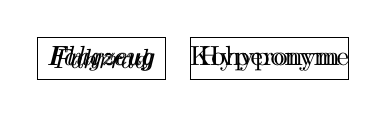
\begin{tikzpicture}
	\Tree [ .\node (level0-right) {\fbox{\textit{Fahrzeug}}}; [ .\node (level1-left) {\textit{Fahrrad}}; ] [ .{\textit{Auto}} ] [ .{\textit{Schiff}} ] [ .{\textit{Zug}} ] [ .\node (level1-right) {\textit{Flugzeug}}; ] ]
	\foreach \Value/\Text in {0/{\fbox{Hyperonym}},1/{Kohyponyme}}
	{
	\node[anchor=west] 
	at ([xshift=1cm]{level1-right}|-{level\Value-right}) 
	{\Text};
	}
\end{tikzpicture}
\end{frame}

\begin{frame}{Hyponymie}
\onslide<+->
jedoch relativer Begriff
\begin{itemize}[<+->]
	\item		d.\,h. grundsätzlich rekursiv
\end{itemize}
\onslide<+->
\Zeile
denn
\begin{itemize}[<+->]
	\item		\textit{Schiff}~\textsubscript{\gruen{Hyponym~1}} natürlich eine Art von \textit{Fahrzeug}~\textsubscript{\alert{Hyperonym~1}}
	\item		aber \textit{Segelschiff}~\textsubscript{\gruen{Hyponym~2}} wieder eine bestimmte Art von \textit{Schiff}~\textsubscript{\alert{Hyperonym~2}}
	\item		{[\ldots]}
\end{itemize}
\end{frame}

\begin{frame}{Hyponymie}
\onslide<+->
\center
\tikzset{level distance=40pt,sibling distance=5pt}
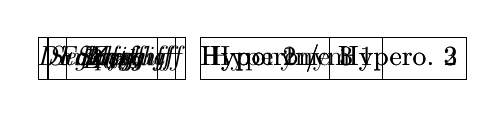
\begin{tikzpicture}
	\Tree [ .\node (level0-right) {\fbox{\textit{Fahrzeug}}}; [ .\node (level1-left) {\textit{Auto}}; ] [ .\node {\fbox{\textit{Schiff}}}; [ .\node (level2-left) {\textit{Dampfschiff}}; ] [ .\node (level2-right) {\fbox{\textit{Segelschiff}}}; [ .\node (level3-left) {\textit{Bark}}; ] [ .{\textit{Galeone}} ] [ .\node (level3-right) {\textit{Brigg}}; ] ] ] [ .\node (level1-right) {\textit{Zug}}; ] ]
	\foreach \Value/\Text in {0/{\fbox{Hyperonym~1}},1/{{Hypo.~1}~/ \fbox{\gruen{Hypero.~2}}},2/{\gruen{Hypo.~2}~/ \fbox{{\alert{Hypero.~3}}}},3/{\alert{Hyponyme~3}}}
	{
	\node[anchor=west] 
	at ([xshift=1cm]{level1-right}|-{level\Value-right}) 
	{\Text};
	}
\end{tikzpicture}
\end{frame}

\begin{frame}{Hyponymie}
\onslide<+->
zugrundeliegende Kategorisierung aber flexibel
\begin{itemize}[<+->]
	\item		sodass Hyponymie von semantischer Vorentscheidung abhängig
	\item		also welche Eigenschaft in Fokus gerückt wird
\end{itemize}
\onslide<+->
\Zeile
denn
\begin{itemize}[<+->]
	\item		nicht nur \textit{Segelschiff}~\textsubscript{\gruen{Kohyponym}} und \textit{Dampfschiff}~\textsubscript{\gruen{Kohyponym}} eine Art von \textit{Schiff}~\textsubscript{\alert{Hyperonym~1}}
	\item		sondern auch \textit{Kriegsschiff}~\textsubscript{\gruen{Kohyponym}} und \textit{Handelsschiff}~\textsubscript{\gruen{Kohyponym}} eine Art von \textit{Schiff}~\textsubscript{\alert{Hyperonym~1}}
	\item		\textit{Kriegsschiff}~\textsubscript{\gruen{Kohyponym}} wiederum mit \textit{Kampfflugzeug}~\textsubscript{\gruen{Kohyponym}} auch eine Art von \textit{Waffensystem}~\textsubscript{\alert{Hyperonym~2}}
	\item		{[\ldots]}
\end{itemize}
\end{frame}

\begin{frame}{Hyponymie}
\onslide<+->
auch bei Verben möglich
\begin{itemize}[<+->]
	\item		allerdings weniger eindeutig als bei Substantiven
	\item		im Vergleich weniger stark ausgeprägt
\end{itemize}
\onslide<+->
\Zeile
\begin{exe}
	\ex\label{ex:hyponymie-003}
    \begin{xlist}
		\ex{\label{ex:hyponymie-003a}		fortbewegen ― rennen, kriechen [\ldots]}
		\onslide<+->
		\ex{\label{ex:hyponymie-003b}		sterben ― verhungern, verdursten [\ldots]}
	\end{xlist}
\end{exe}
\end{frame}



\section{Ausblick}

\begin{frame}{Architektur des Wortschatzes}
\onslide<+->
\begin{itemize}[<+->]
  \item weitere Sinnrelationen (Kontiguität, \ldots)
	\item	Wortfelder
	\item	Wortfamilien
\end{itemize}
 \end{frame}
 
 %Markiertheit, markiert hinsichtlich
 %varietätenspezifische Wortschätze

